\chapter{Chirality: Molecular Hands Are Not Always Equal}

\begin{kaichang}
Try two small things.

First, if you have an orange and lemon, peel a little skin from each, fold it outward, and smell the released mist. Eyes closed, you can distinguish the scents. Would you believe their leading aroma molecules have identical composition and connectivity, differing only as mirror images?

Second, try a left glove on your right hand. No wrist rotation makes it fit. Both hands contain the same bones and joints, so why are they not interchangeable?

Write down both puzzles. By the end, citrus peel, gloves, and a tragedy that changed drug regulation worldwide will reveal one shared rule: \textbf{mirror images are not always equivalent}.
\end{kaichang}

\section{Start with a Pair of Gloves}

Why does a left glove not fit the right hand? Rather than dismiss it as obvious, compare carefully. Stack both hands palm-down: fingertips match, but thumbs point opposite ways. Flip one to align thumbs, and palm and back mismatch. Like objects in a mirror, they look identical yet never fully overlap.

Geometry calls this nonsuperimposable mirror images. Everyday examples abound:

\begin{itemize}[itemsep=2pt]
\item Screw threads can be right- or left-handed: right-handed screws tighten clockwise, left-handed the reverse. Gas-cylinder fittings deliberately use left-handed threads so their special status is immediately apparent by eye or hand.
\item Most freshwater snail shells coil rightward; rare left-coiled individuals are collectors' treasures.
\item Springs, spiral stairs, and morning-glory vines have handed winding directions; reversing one makes something different.
\end{itemize}

Their difference is not material but three-dimensional arrangement. Left and right shoes share leather and rubber; space carries the difference.

But molecules are hundreds of millions of times smaller than gloves, beyond sight or touch. How can we claim molecular hands? This chapter searches for that invisible glove.

\section{Zoom In: Four Different Neighbors}

At molecular scale, recall Chapters 19 and 20: carbon's four covalent bonds point not flatly but to a \textbf{tetrahedron}'s vertices, carbon at the center and a neighbor at each corner.

Fill those corners for lactic acid, yogurt's main sour ingredient. Its central carbon joins hydrogen, H; hydroxyl, \chem{OH}; methyl, \chem{CH_3}; and carboxyl, \chem{COOH}. \textbf{All four neighbors differ.}

Build this mentally, placing the groups arbitrarily at four corners. Swap any two. Is the new arrangement the same thing?

Rotate it as you like: it never fully overlaps the original, just as wrist rotation cannot fit the wrong glove. The models are nonsuperimposable mirror images, called \textbf{enantiomers}, paired mirror forms. The central carbon with four different groups is a \textbf{chiral center}, and molecular handedness is \textbf{chirality}, from Greek for hand.

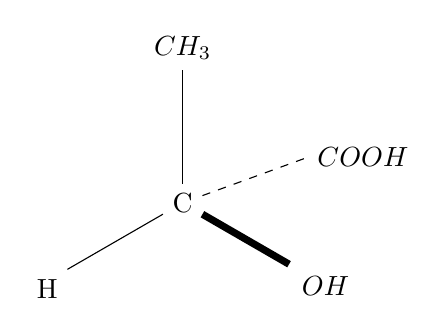
\begin{tikzpicture}[scale=1.3]
  \node (c) at (0,0) {C};
  \draw (c) -- (90:1.3) node[above] {$\chem{CH_3}$};
  \draw (c) -- (210:1.3) node[below left] {H};
  \draw[line width=2.6pt] (c) -- (330:1.2) node[below right] {$\chem{OH}$};
  \draw[dashed] (c) -- (20:1.3) node[right] {$\chem{COOH}$};
\end{tikzpicture}

This is chemists' tetrahedral-carbon convention: ordinary thin lines lie in the paper; a \textbf{thick wedge} projects toward you; a \textbf{dashed line} recedes behind. It is a human-made representation: molecules have no colors and bonds are not sticks. Build four toothpicks in clay, then swap two, to feel the inability to rotate back.

Remember three points. First, enantiomers have the same composition and even the same atom connections; only their spatial arrangements differ. Second, to test a carbon center, check whether all four neighbors differ. Any matching pair, such as ethanol's two hydrogens, lets the mirror images overlap and removes molecular chirality. Third, chirality is not exclusive to carbon, though tetrahedral carbon is its commonest source.

\section{Ordinary Methods Cannot Tell; Polarized Light Can}

How alike are enantiomers? The two lactic acids share melting point, boiling point, water solubility, density, and reaction rates with ordinary reagents. Chapter 3's distillation, crystallization, and filtration cannot separate them. Unsurprising: physical properties largely follow size, polarity, and intermolecular attraction (Chapter 22), identical for mirrored hands.

But one kind of light distinguishes them.

Ordinary light vibrates in all directions. Pass it through a polarizer, such as a sunglasses lens, and only one vibration direction remains, like a rope wave passing vertical railings: \textbf{polarized light}. Early nineteenth-century physicists found sugar solution \textbf{rotates} its vibration plane. An invisible hand seems to twist the light, more strongly with higher concentration and longer paths. This is \textbf{optical activity}.

One enantiomer twists left, the other right, by \textbf{equal angles in opposite directions}. Equal mixtures cancel, producing no rotation: a \textbf{racemate}. A polarimeter measures rotation and remains routine in pharmaceutical quality control.

\begin{shiyan}
\textbf{See Light Twist at Home}

Materials: a clear glass; clean water; two spoonfuls of honey or corn syrup; two polarizers, such as old passive 3D-glasses lenses or polarized sunglasses; a phone or computer LCD screen.

Procedure: display a pure-white image; LCD light is already polarized. View it through a polarizer and rotate slowly until nearly black, noting the position. Then place the glass of thoroughly mixed sugar solution, about one-third full, between lens and screen.

What to observe: the dark screen brightens! Rotate the viewing polarizer further to darken it again; that angle measures the sugar solution's rotation. Try clean water: it stays black, since water molecules are achiral.

Safety: never look directly at the Sun through the lenses. Handle glass gently. Honey is sticky; wash hands and wipe the table afterward.
\end{shiyan}

Sugar molecules twisted the light you just adjusted. Sugars are chiral (Chapter 46), and honey's sugars all share the same hand, a point we will revisit.

\section{Pasteur's Tweezers}

\begin{zhengju}
Molecular handedness was forced upon scientists by a jar of crystals, not invented at whim. The protagonist was twenty-six-year-old French chemist Pasteur, later famous for pasteurization, whose scientific career began with crystals.

In 1848, he studied tartaric acid, a winemaking byproduct. One puzzle was known: wine-derived tartaric acid rotated polarized light in solution, while chemically identical racemic tartaric acid did not. Same composition, different rotation, unexplained by existing theory.

Pasteur noticed a detail predecessors left: small crystal faces appeared only on one side of tartrate crystals, like a glove's thumb. If molecules had hands, perhaps crystals did too. He slowly crystallized racemic sodium ammonium tartrate at low temperature, then used tweezers under a microscope to sort crystals individually by face orientation into left and right piles.

Separate solutions in the polarimeter rotated equally in opposite directions. Nonrotating racemic tartaric acid had contained equal proportions of oppositely rotating crystals! Pasteur recalled rushing from the laboratory in excitement and embracing the first person in the corridor.

Three lessons deserve thought. First, not a guess of chirality but a testable prediction: equal opposite rotations, decided by instruments. Second, alternatives were excluded. If crystal shape alone caused rotation, dissolution should remove it; rotation persisted, placing chirality in molecules. Third, luck mattered: only below about $28\,^{\circ}\mathrm{C}$ does this salt form separate handed crystals. Above, both molecules join identical crystals beyond tweezers' power. A midsummer experiment might have changed history.

Why do molecular hands arise? In 1874, van 't Hoff and Le Bel independently proposed tetrahedral carbon: four distinct neighbors at four corners, with nonsuperimposable mirrors. Many mocked the unseen tetrahedron as fantasy. Decades later, X-ray crystallography directly measured atom positions and found it exactly.
\end{zhengju}

\section{Naming Left and Right}

Now symbols enter. Chemists give enantiomers two sets of names.

One follows optical rotation: rightward $(+)$, formerly d; leftward $(-)$, formerly l. Intuitive, but it says where light turns, not how atoms are arranged.

The other names arrangement itself. Rank four neighbors by priority and view by defined rules: clockwise gives $(R)$, Latin right; counterclockwise gives $(S)$, Latin left. Details belong to the challenge. For the main thread, $(R)$ and $(S)$ describe appearance, with \textbf{no simple correspondence} to optical rotation: some $(R)$ molecules are $(+)$, others $(-)$. Confusing these schemes is a common beginner's trap.

Lactic acid is therefore $(S)$-$(+)$ or $(R)$-$(-)$. Almost all lactic acid in exercised muscles and yogurt is one form; ordinary laboratory synthesis gives equal racemic amounts. Why does life make only one hand? That comes later.

\section{Noses, Medicines, and Enzymes Distinguish Hands}

Now answer the opening question: if physical properties match, how can your nose distinguish orange and lemon?

Pairing explains it. A chiral glove fits only its matching hand. Olfactory receptors are proteins, themselves highly chiral molecular machines, detailed in Chapter 48. When orange-peel limonene enters, $(R)$-limonene fits one receptor and smells orange; mirrored $(S)$-limonene fits awkwardly, triggering another receptor set for lemon-and-pine-like scent. \textbf{Same composition and connections, different smells from mirror images}, because your nose is chiral.

Spearmint and caraway, familiar flavorings in gum and Western food, offer another pair: carvone enantiomers smell cool and minty or spicy like fennel seeds.

Medicines make the same point more seriously. Drugs usually fit protein cavities like keys in chiral locks, where mirrored keys often fail. Ibuprofen's main anti-inflammatory form is $(S)$. Fortunately, the body slowly converts some ingested $(R)$ to $(S)$, so pharmacy racemic ibuprofen works, reminding us that mirrored molecules need not remain unchanged inside. Parkinson's medicine levodopa carries chirality in its name: only the left form crosses the blood--brain barrier and is used by nerve cells; the mirror is almost ineffective.

Enzymes are selectivity's extreme. An enzyme lock often recognizes just one substrate hand, with the mirror reacting thousands of times slower or not at all (Chapter 49). Drug manufacturers therefore either make only the needed hand or laboriously separate a mixture, a major modern pharmaceutical cost.

\section{Thalidomide: A Story That Must Be Told Fully}

Chirality lessons nearly always mention thalidomide, marketed in China as Fan Ying Ting, often compressed into right-handed medicine, left-handed poison, and safety after banning the bad hand. Reality is more complicated and instructive. Take it slowly.

In 1957, West Germany's Grünenthal launched thalidomide as a sedative, advertised as safe even in pregnancy. It soon sold over the counter for morning sickness in dozens of countries. Regulation then matters: most countries required manufacturers only to show it did not kill, \textbf{not test effects on pregnant people or fetuses}, nor demonstrate effectiveness. Animal testing was cursory, with no pregnancy testing at all.

The United States was an exception, but fortuitously so. Under a 1938 law, new drugs required FDA safety review. Reviewer Frances Kelsey found the submitted safety evidence thin, particularly for pregnancy and long-term use, and resisted repeated company pressure to approve. Through 1960 and 1961, thalidomide remained off the US market.

In 1961, Germany's Lenz and Australia's McBride raised alarms: unusual limb defects, phocomelia, suddenly clustered with timelines closely matching early-pregnancy thalidomide exposure. By year's end, countries began withdrawals. More than ten thousand infants worldwide were born with lifelong disabilities, while Kelsey's delay left relatively few US cases. The next year, Congress amended the law to require both \textbf{safety and effectiveness}, and postmarketing adverse-effect monitoring gradually developed internationally. The tragedy shaped today's regulatory system.

Now tell the stereochemistry fully. Thalidomide has one chiral center. Animal work associates $(S)$ more strongly with fetal-development harm; in 2010 scientists identified its target, cereblon, to which $(S)$ binds more tightly. Does the popular slogan now seem right?

No. Two omitted facts are crucial. First, the enantiomers \textbf{rapidly interconvert} at body temperature and blood acidity, becoming a half-and-half racemate within hours. Even pure $(R)$ sold then would have produced abundant $(S)$ after ingestion. Second, detailed research shows overlapping pharmacology, not entirely good versus entirely bad forms. Blaming bad chirality both misstates chemistry and conceals the lesson: \textbf{the real failure was missing pregnancy-evidence requirements and unsupported safety claims}. Kelsey blocked not a bad molecular half, but an entire untested drug package.

The ending is counterintuitive too: thalidomide did not enter history's dustbin. In 1964, a doctor treated a severe inflammatory leprosy complication with striking results. In 1998, FDA reapproved it with extremely strict controls, compulsory contraception for reproductive-age patients and prescription tracking. Today it also remains important for multiple myeloma. One molecule can be disastrous for one purpose and valuable for another: evidence, dose, patient population, and regulation decide, not labels of good or bad.

\begin{qiaoliang}
Use numbers to challenge the idea that sufficient purity excludes the other hand.

A 100 mg thalidomide tablet, molar mass about \ud{258}{g\cdot mol^{-1}}, contains $0.1\div258\approx3.9\times10^{-4}$ mol. Multiply by Avogadro's constant, \ud{6.02\times10^{23}}{mol^{-1}} from Chapter 5, to obtain about $2.3\times10^{20}$ molecules, twenty quintillion.

Even astonishing 99.99\% purity leaves one mirror impurity per ten thousand molecules. Calculate $2.3\times10^{20}\times0.0001=2.3\times10^{16}$: \textbf{still over ten quadrillion} mirror molecules, before bodily interconversion. High purity matters, but an absolutely pure hand does not exist in molecular reality. Evidence standards and monitoring truly protect patients.
\end{qiaoliang}

\section{Why Is Life Uniformly Left-Handed?}

Bring out the fifth recurring question: how does life preserve, copy, regulate, and select chirality?

Consider this striking list: amino acids in your proteins are almost uniformly L, while DNA sugars uniformly use the other designation, D. Not 99\%, but nearly 100\%: billions of species from bacteria to blue whales follow one chiral constitution, copied for billions of years.

Why is uniformity needed? A protein is an intricately folded amino-acid machine (Chapter 48). Mix left and right parts along its chain and the shape becomes disordered, wrecking the machine. Again, the whole production line must use the same glove mold.

Why specifically L amino acids and D sugars, not the reverse? Honestly, \textbf{we do not know}. Clues exist. Some meteorites contain small L excesses of certain amino acids, showing space chemistry can create handed biases. Laboratory self-amplifying reactions let a slight excess catalyze more of its own hand, snowballing. Physicists note that the weak interaction, one of four fundamental forces, distinguishes left and right, creating exceedingly small mirror-energy differences. These clues are real, but no accepted answer identifies the dominant cause or complete causal chain. Unfinished scientific questions show science is alive; Chapter 87 returns to such mysteries.

\section{Where Does This Model Fail?}

Four different neighbors around carbon is a powerful model. Knowing its limits completes understanding.

\begin{itemize}[itemsep=2pt]
\item \textbf{Chiral centers do not guarantee a chiral molecule}. Tartaric acid has two, yet one form twists them oppositely and has an internal mirror plane, like wearing the wrong glove on each hand. The whole overlaps its mirror and is a nonrotating meso compound. This third route completes Pasteur's tartaric-acid family.
\item \textbf{Molecules without chiral centers can be chiral}. Substituted allenes have perpendicular terminal groups, making a twisted-towel arrangement with hands; helical molecules have handed spirals themselves.
\item \textbf{A chiral center can be dismantled}. Thalidomide teaches that any chemically accessible inversion path lets mirrors mix equally on timescales from seconds to hours. Retaining a hand depends not only on a structural drawing but chemistry in the actual environment.
\item \textbf{Enantiomer differences appear only in chiral surroundings}. Ordinary achiral solvents, reagents, and physical measurements treat both alike. Differences emerge on meeting another hand, polarized light, chiral receptors, or enzymes. Thus identical properties hold in a vacuum, not in your body.
\end{itemize}

\begin{wuqu}
``Enantiomers differ only in optical-rotation direction; everything else is identical.''

First counterexample: carvone's spearmint and caraway smells imply different receptor binding. Second: levodopa works while its mirror nearly does not. Third: enzymes often catalyze only one hand, with hundredfold or thousandfold rate differences.

Correctly stated, enantiomers share physical and chemical properties in an \textbf{achiral environment}, including melting, boiling, and ordinary solubility. In \textbf{chiral environments}, polarized light, receptors, enzymes, and catalysts, differences can determine life or death. Life itself is the most selective chiral environment.
\end{wuqu}

\section{Back to Citrus Peel and Gloves}

Now fulfill the opening promise.

Orange-peel mist mainly contains $(R)$-limonene; lemon peel and turpentine mainly its mirror, $(S)$-limonene. Composition and connections match and ordinary physical properties hardly distinguish them, but your protein receptor gloves feel different hands differently, producing orange and lemon smells. Distinguishing fruit aromas blindfolded is a precise chiral-recognition experiment.

The wrong glove follows the same geometry as lactic acid, limonene, and thalidomide: identical parts, nonsuperimposable mirror arrangements, no interchangeability. Hand and nose puzzles echo across scales.

The opening's third hidden subject was a world-changing drug tragedy. Thalidomide's mirror differences are real, but the lesson is not poisonous left hands. When chemical complexity, bodily interconversion and target binding, meets absent evidence standards, those least protected by the evidence chain suffer: then, fetuses not yet born.

\section{Making One Hand Industrially}

Understanding chirality is for mastering it, not contemplating tragedy. Modern pharmaceuticals have two tools.

First, \textbf{asymmetric catalysis}. If ordinary synthesis yields half-and-half racemates, make the catalyst chiral: reactions in handed molds favor one product hand. The 2001 Chemistry Nobel honored pioneers: Knowles industrialized levodopa this way, Noyori raised efficiency to industrial levels, and Sharpless made a broad class of oxidations selectively handed. Menthol, antibiotics, blood-pressure drugs, and many other products use chiral catalysis or chromatographic resolution of mirrors.

Second is regulation's legacy: approval now requires separately understanding each enantiomer's absorption, conversion, and toxicology, a memorial to thalidomide written into institutions.

A larger question emerges. Receptors and enzymes are chiral, DNA and proteins use handed components, but what are those components? Why do proteins fold into gloves recognizing only one hand? How do enzymes recognize in milliseconds? The next part crosses from molecular arrangement to molecular life. Your twenty amino acids are coming, after Chapter 46's sugars, with proteins in Chapter 48 and enzymes in Chapter 49. Each carries today's hand.

\begin{tiaozhan}
How are $(R)$ and $(S)$ assigned? CIP priority rules have three steps. First, rank four groups by directly attached atom's atomic number: oxygen of \chem{OH} $>$ carbon of \chem{COOH} $>$ carbon of \chem{CH_3} $>$ H. Break ties by successive atom layers. Second, point the lowest-priority group away, into the paper. Third, follow the remaining three from highest to lowest: clockwise $(R)$, counterclockwise $(S)$.

Practice lactic acid: \chem{OH} $>$ \chem{COOH} $>$ \chem{CH_3} $>$ H. With H away, counterclockwise \chem{OH} $\rightarrow$ \chem{COOH} $\rightarrow$ \chem{CH_3} is $(S)$, the lactic acid in muscle. Counterintuitively, this wholly human convention has no formula linking it to optical direction. $(S)$-lactic acid is $(+)$, yet some $(S)$ molecules are $(-)$. Naming and rotation are separate, illustrating science's define-first-then-use convention. Skipping this box leaves the thread intact.
\end{tiaozhan}

\section*{Try It Yourself}

\begin{sikaoti}
\item Build lactic acid's two enantiomers with toothpicks and clay, or draw with wedge--dash notation. Mark the center, rotate one several ways, and explain why it never overlaps the other. Note that representations aid thinking; real bonds are not sticks.
\item Identify chiral carbons in ethanol, \chem{CH_3CH_2OH}; lactic acid, \chem{CH_3CH(OH)COOH}; and glycerol, \chem{HOCH_2CH(OH)CH_2OH}. Count four neighbors for each.
\item Diagram the home experiment's light path: LCD, sugar glass, polarizer. Mark polarization changes at each step and explain why clean water leaves the screen black.
\item A racemate contains equal enantiomers. If individual molecules rotate light, why does the whole solution not? Explain with each molecule twisting the light.
\item Tartaric acid has two chiral centers but a nonrotating meso form. Explain or sketch why centers do not guarantee molecular chirality. Hint: think of a person wearing opposite gloves on both hands.
\item A drug-company spokesperson claims 100\% pure $(R)$-thalidomide is therefore absolutely safe. Refute this with two chapter facts and state what is genuinely missing.
\end{sikaoti}
